%%%%%%%%%%%%%%%%%%%%%%%%%%%%%%%%%%%%%%%%%%%%%%%%%%%%%%%%%
%                                                       %
%  			 MASER				%
%                                                       %
%%%%%%%%%%%%%%%%%%%%%%%%%%%%%%%%%%%%%%%%%%%%%%%%%%%%%%%%


\documentclass[a4paper,12pt]{article}
%Fichero con configuración opcional:
%
% Paquetes que pueden serte de utilidad (rec = recomendado, opc = opcional)
%
\usepackage{fancyhdr}          % (rec)  permite cambiar varios par�metros de las cabeceras y pi�s de p�gina
\usepackage{fancyvrb}		% (rec) permite cambiar parámetros del texto
% literal (entorno verbatim)
\usepackage{courier}           % (opc)  usa esta fuente por defecto
\usepackage[spanish]{babel}   % (rec)  da soporte para castellano a LaTeX
\usepackage[utf8]{inputenc}    % (rec) soporte para tildes
%\usepackage{setspace}          % (opc)  permite cambiar el espaciado entre l�neas
%\usepackage{longtable}         % (opc)  permite que las tablas ocupen varias p�ginas
%\usepackage{lscape}            % (opc)  permite el uso del comando \landscape, para poner algo apaisado
\usepackage{color}             % (opc)  varios comandos relativos al color (como
% \color)
% \usepackage{colortbl}           % (opc) permite usar color en las tablas
% \usepackage{rotating}          % (opc)  permite rotar PSs y EPSs
% \usepackage{textcomp}          % (opc)  permite incluir el s�mbolo del euro,
% con \texteuro
%\usepackage{minitoc}           % (opc)  permite incluir ToCs (�ndice de materias) para cada cap�tulo
%\usepackage{epsf}              % (opc)  permite ciertas manipulaciones a EPSs
\usepackage[absolute]{textpos} % (rec)  permite posicionado arbitrario de texto (necesario para la portada)
%\usepackage{srcltx}            % (opc)  permite pasar del .dvi al .tex
% \usepackage{marvosym}
\usepackage[breaklinks=true, colorlinks]{hyperref} % (opc) hace que las
% referencias cruzadas se conviertan en enlaces
% \usepackage{titleref}           % (opc) permite hacer referencia a otra
% sección mostrando su título
\usepackage{graphicx}
% \usepackage{multirow}
% \usepackage{setspace}
\usepackage{url}     % Enlaces web
% \usepackage{tabularx} %Ajuste automático del ancho de columnas
% \usepackage{longtable} %Tablas de más de una página, por ejemplo para los
% acrónimos
\usepackage{listings} %Mostrar código en el texto, por ejemplo comandos de consola
\usepackage{cmap}   %Hacer que el pdf sea searchable

\pretolerance=10000 %Para evitar que se corten las palabras
\tolerance=10000  %Para evitar que se corten las palabras
\usepackage[scaled=0.92]{helvet}
\renewcommand{\sfdefault}{phv} %para cambiar el tipo de fuente por defecto
%Comando para configurar el documento en Arial
\sffamily %trabaja con helvetica en el cuerpo del documento
\renewcommand{\rmfamily}{phv} % permite trabajar con helvetica los títulos
\renewcommand{\familydefault}{phv} % permite trabajar con letra helvetica los títulos

\definecolor{gray97}{gray}{.97}
\definecolor{gray75}{gray}{.75}
\definecolor{gray45}{gray}{.45}
 
\lstset{ frame=Ltb,
     framerule=0pt,
     aboveskip=0.5cm,
     framextopmargin=3pt,
     framexbottommargin=3pt,
     framexleftmargin=0.4cm,
     framesep=0pt,
     rulesep=.4pt,
     backgroundcolor=\color{gray97},
     rulesepcolor=\color{black},
	inputencoding=utf8,
	extendedchars=\true,
     %
     stringstyle=\ttfamily,
     showstringspaces = false,
     basicstyle=\small\ttfamily,
     commentstyle=\color{gray45},
     keywordstyle=\bfseries,
     %
     numbers=left,
     numbersep=15pt,
     numberstyle=\tiny,
     numberfirstline = false,
     breaklines=true,
     escapeinside=+ +,
   }
 
% minimizar fragmentado de listados
\lstnewenvironment{listing}[1][]
   {\lstset{#1}\pagebreak[0]}{\pagebreak[0]}
 
\lstdefinestyle{consola}
   {basicstyle=\scriptsize\bf\ttfamily,
    backgroundcolor=\color{gray75},
   }

\lstdefinestyle{archivo}
   {basicstyle=\scriptsize\ttfamily,
    backgroundcolor=\color{gray97},
   }

%\usepackage{urlbst} %Soporte para url en bibtex
%
% Settings para los m�rgenes. Descomenta y modifica si sabes lo que haces. N�tese
% que a los valores dados se les a�ade una pulgada extra. Los valores dados son los
% predeterminados para papel A4 y el estilo itsas_pfc.cls.
%
%\setlength{\oddsidemargin}{10pt}     % m�rgen izquierdo para p�ginas impares (izquierda)
%\setlength{\evensidemargin}{52pt}    % m�rgen izquierdo para p�ginas pares (derecha)
%\setlength{\textwidth}{390pt}        % anchura del cuerpo de texto

%
% Recomendado para mejorar la colocaci�n autom�tica de las figuras.
% (tomado de http://dcwww.camp.dtu.dk/~schiotz/comp/LatexTips/LatexTips.html#captfont)
%
\renewcommand{\topfraction}{0.85}
\renewcommand{\textfraction}{0.1}
\renewcommand{\floatpagefraction}{0.75}

%
% Espacio entre el borde superior de la p�gina y donde comienza el texto (ah� van las
% cabeceras). LaTeX se queja si usamos el paquete fanchyhdr y headheight es menor de 15pt
%
\headheight 16pt

%
% Para el paquete textpos (usado para la portada)
%
\setlength{\TPHorizModule}{\paperwidth}
\setlength{\TPVertModule}{\paperheight}
\newcommand{\tb}[4]{\begin{textblock}{#1}[0.5,0.5](#2,#3)\begin{center}#4\end{center}\end{textblock}}

\newcommand{\respuesta}[1]{\setlength{\parindent}{0pt}\colorbox[gray]{0.87}{\scriptsize\texttt{\BUseVerbatim{#1}}}\setlength{\parindent}{1cm}}

%
% Aqu� puedes definir tus comandos.
% 
% \newcommand{cmd}[args]{def}
%
% cmd  = el comando a definir (p.e. \cadena)
% args = el n�mero de argumentos
% def  = la definici�n, sustituyendo #1, #2... por el primer, segundo... argumento
%
% Por ejemplo:
%
% \newcommand{\agua}[1]{H\ensuremath{_#1}O}
%
% Cada vez que escribamos "\agua{33}", en el output saldr�: "H33O" (con el 33 como sub�ndice)
%

%\newcommand{\algo}{algo}
% 
% \newcommand{\todolist}[1]{
%  \marginpar{
%   \fbox{
%    \begin{minipage}{3cm}
%     \tiny{
%      \begin{list}{$\bullet$}
%       {
%       \textsc{\textbf{To do: }}\vspace*{-0.2cm}
%       \setlength\labelwidth{0.1cm}
%       \setlength\itemindent{0cm}
%       \setlength\leftmargin{0.05cm}
%       \setlength\parsep{0cm}
%       \setlength\itemsep{0.05cm}
%       }
%       #1
%      \end{list}
%     }
%    \end{minipage}
%   }
%  }
% }

%
% Aqu� puedes instruir a LaTeX de por d�nde cortar las palabras que �l autom�ticamente
% no sepa. P.e., para cortar "gnomonly" solo por donde se se�ala con guiones (-).
%
% \hyphenation{gno-mon-ly} 
 
%
% Que las primeras p�ginas sean numeradas con n�meros romanos.
% M�s adelante se cambiar� de nuevo a ar�bicos.
%
\pagenumbering{Roman}


\begin{document}
%Da valores a ciertas variables:
%
% Este fichero contiene una lista de nombres (variables) internos
% de LaTeX, a los que puedes cambiar el nombre. Por ejemplo, puedes
% hacer que los cap�tulos se llamen "Secci�n" en vez de "Cap�tulo"
%
\renewcommand\bibname{Bibliograf\'{\i}a}        % as� el nombre de la secci�n Bibliograf�a ser� "Bibliograf�a".
\newcommand{\myname}{Digna González Otero}                 % nombre del autor.
\newcommand{\myboss}{José Daniel Gutiérrez Porset}                 % nombre del supervisor.
\newcommand{\thesistitle}{\uppercase{Construcción e implantación de herramientas para la gestión colaborativa del conocimiento en el GSC}}        % t�tulo del trabajo.
\newcommand{\worktype}{Proyecto Fin de Carrera} % tipo de trabajo.
\newcommand{\upv}{Utils/ehu_logo.eps}          % fichero con el logo (p.e. para la portada).
\newcommand{\ibi}{Utils/logo_ingenieria.eps}          % fichero con el logo (p.e. para la portada).
\newcommand{\logoupv}{Utils/ehu_logo.png}          % fichero con el logo (p.e. para la portada).
\newcommand{\logoibi}{Utils/logo_ingenieria.png}          % fichero con el logo (p.e. para la portada).
%\renewcommand{\figurename}{xxx}                % nombre a pie de figura (xxx 1: bla-bla-bla).
%\renewcommand{\listfigurename}{yyy}            % nombre del �ndice de figuras.
\renewcommand{\tablename}{Tabla}
\renewcommand{\listtablename}{Índice de tablas}

    \makeatletter
    \def\thebibliography#1{\section*{REFERENCIAS\@mkboth
      {REFERENCIAS}{REFERENCIAS}}\list
      {[\arabic{enumi}]}{\settowidth\labelwidth{[#1]}\leftmargin\labelwidth
	\advance\leftmargin\labelsep
	\usecounter{enumi}}
	\def\newblock{\hskip .11em plus .33em minus .07em}
	\sloppy\clubpenalty4000\widowpenalty4000
	\sfcode`\.=1000\relax}
    \makeatother

%Página de portada:
%
% Este fichero produce la primera p�gina del PFC/Tesis, con el
% t�tulo, tu nombre, el nombre del supervisor, etc.
%
% La mayor�a, si no todo el contenido de esta p�gina est� incluido a trav�s 
% de comandos (p.e. \thesistitle) que han sido definidos en Config/pfc_options.tex
%
% Editar a voluntad.
%

\thispagestyle{empty} % no imprimir ni n�mero, ni cabecera ni pi� de p�gina

%
% Usa \tb para colocar varios items en la p�gina. Uso:
%
% \tb{w}{h}{v}{t}
%
% donde:
%
% w = ancho de la caja con el texto (1.0 = ancho de p�gina)
% h = posici�n horizontal del centro de la caja de texto (0.0 = izquierda, 1.0 = derecha)
% v = posici�n vertical del centro de la caja de texto (0.0 = arriba, 1.0 = abajo)
% t = texto a incluir en la caja de texto
%
\tb{0.4}{0.25}{0.1}{\includegraphics[width=0.8\textwidth]{\logoupv}} % logo UPV/EH
\tb{0.6}{0.7}{0.1}{\includegraphics[width=0.65\textwidth]{\logoibi}} % logo UPV/EHU
%
\includegraphics[width=0.5\textwidth]{Utils/ehu_logo.png}
\tb{0.8}{0.5}{0.17}{\rule{\columnwidth}{0.025cm}}
%%\tb{0.8}{0.50}{0.40}{\Large \worktype}                        % si es PFC o Tesis
\tb{0.5}{0.50}{0.30}{\huge Circuitos de Alta Frecuencia}
\tb{0.8}{0.50}{0.40}{\large {4º CURSO DE INGENIERÍA DE TELECOMUNICACIÓN}}
\tb{0.8}{0.50}{0.50}{\large{AÑO ACADÉMICO:	2009/2010}}
\tb{0.8}{0.50}{0.60}{\huge MASER:}
\tb{0.8}{0.50}{0.67}{\large{\textbf{Microwave Amplification by Stimulated Emission of Radiation }}}
\tb{0.8}{0.70}{0.85}{Digna María González Otero\\Iv\'an Iglesias de Lama}

\ \clearpage                       % terminar la p�gina aqu�%
\thispagestyle{empty} \ \clearpage % p�gina en blanco

% CONFIG: Inicializar en 1 el n�mero de p�gina
%% Usa \cdpchapter para todos los cap�tulos que comienzen "a la derecha"
% Y no tienen n�mero (p.e. los Agradecimientos):
\newcommand{\cdpchapter}[1]{\cleardoublepage\chapter*{#1}}

% Comienza a contar las p�ginas de 1 otra vez:
\setcounter{page}{1}

% CONFIG: �ndice de materias (ToC)
%\dominitoc        % que cada cap�tulo tenga su ToC (necesita el paquete "minitoc" antemencionado)
\tableofcontents  % insertar ToC en este punto
%\newpage
%\listoffigures    % insertar lista de Figuras (LoF) en este punto (opcional)
%\newpage
%\listoftables     % insertar lista de Tablas (LoT) en este punto (opcional)

\cleardoublepage

% CONFIG: Definir el estilo de las cabeceras/pi�s de p�gina.
\pagestyle{fancy}                                % elegir este estilo de cpps (recomendado)
\fancyhf{}                                       % borra el estilo anterior para cpps, para luego redefinirlos
\fancyfoot[C]{\textbf{\thepage}}             % Cabecera: n�mero de p�gina en negrita.
\fancyhead[R]{\nouppercase{\leftmark}}          % Cabecera: incluye informaci�n del nivel superior (Cap�tulo)
\renewcommand{\headrulewidth}{0.5pt}             % Cabecera: subraya la cabecera (fijar en "0pt" si no se desea).
\renewcommand{\footrulewidth}{0.5pt}               % Pi�: subraya el pie de p�gina (fijar en "0pt" si no se desea).






% CONFIG: Estilo de los cap�tulos

\setlength{\parskip}{0.5cm} %Separación entre párrafos

% Usa \tocchapter en vez de \chapter, para usar cap�tulos
% bien formateados:
%\newcommand{\tocchapter}[1]{\cleardoublepage\chapter{#1}\minitoc\newpage}

% CONTENIDO: Tras esto puedes incluir todos los cap�tulos/secciones que desees.
\section{Introducción}
\label{introduccion}

Un m\'aser es un \textbf{dispositivo que produce ondas electromagn\'eticas coherentes} mediante la amplificaci\'on por la emisi\'on estimulada de radiaci\'on \cite{maserDefinition}. El t\'ermino se defini\'o como acr\'onimo de \textit{Microwave Amplification by Stimulated Emission of Radiation}.

Como su nombre indica, su funcionamiento está basado en el fenómeno de emisión estimulada de radiación, enunciado por Albert Einstein en 1916.

Una de las principales aplicaciones de los m\'aseres es como relojes at\'omicos de gran precisi\'on, pero tambi\'en se usan como amplificadores, principalmente en radiotelescopios. En secciones posteriores de este documento profundizaremos en las aplicaciones de este tipo de dispositivos.

\subsection{Historia}

El funcionamiento del m\'aser est\'a basado en el fen\'omeno de emisi\'on estimulada de radiaci\'on enunciado por Albert Einstein en 1916. 

En mayo de 1952 Nikolay Basov y Alexander Prokhrov del Instituto de F\'isica de Lebedev describieron el principio del m\'aser en la Academia de Ciencias de la URSS. M\'as tarde, en octubre de 1954  publicaron los resultados de su investigaci\'on.

De forma independiente Charles H. Townes, J. P. Gordon y H. J. Zeiger fabricaron en 1953 en la Universidad de Columbia el primer m\'aser. Este dispositivo utilizaba un haz de mol\'eculas de amon\'iaco para producir la amplificaci\'on de microondas a la frecuencia de 24 GigaHerzios.

M\'as tarde Townes trabaj\'o con Arthur L. Schawlow para describir el principio del m\'aser \'optico o l\'aser, y en 1958 hicieron varias publicaciones sobre este tema, aunque por aqu\'el entonces no siguieron con las investigaciones en ese campo.

En 1959 Townes y Schawlow obtuvieron una patente del m\'aser. Este dispositivo se usaba para amplificar se\~nales de radio y como detector ultrasensible para investigaci\'on espacial.

En 1964 Townes, Basov y Prokhorov recibieron el premio Nobel de F\'isica por su trabajo en este campo. A Townes se le adjudic\'o la mitad del premio y la otra mitad se reparti\'o entre Basov y Prokhorov.

\begin{figure}[h]
\begin{center}$
\begin{array}{ccc}
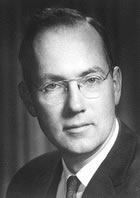
\includegraphics[width=0.25\textwidth]{./Utils/townes.jpg} &
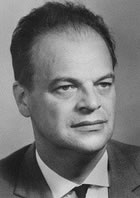
\includegraphics[width=0.25\textwidth]{./Utils/basov.jpg} &
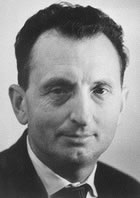
\includegraphics[width=0.25\textwidth]{./Utils/prokhorov.jpg}
\end{array}$
\end{center}
\caption{Townes, Basov y Prokhorov, de izquierda a derecha}
\end{figure}

En 1965 se descrubri\'o el primer m\'aser astron\'omico en la nebulosa de Ori\'on. Era un m\'aser de hidroxilo, que emite radiaci\'on en varias longitudes de onda, aunque las m\'as utilizadas son las de 18cm (1,7GHz de frecuencia).
\subsection{Terminolog\'ia}

Aunque el t\'ermino \textit{MASER} se difini\'o como acr\'onimo de \textbf{Microwave Amplification by Stimulated Emission of Radiation}, con el tiempo y el avance de la tecnolog\'ia este t\'ermino se ha ido quedando obsoleto, y se ha empezado a llamar al dispositivo \textit{m\'aser} en min\'usculas, y ya no en forma de acr\'onimo. 

El motivo por el que la definici\'on ya no es precisa es debido a que el rango de frecuencias de funcionamiento de los m\'aseres actuales no est\'a limitado al de microondas, sino que se extiende en el espectro. Por este motivo el f\'isico Charles H. Townes, quien le hab\'ia dado el nombre original junto con sus colaboradores, sugiri\'o sustituir la palabra ``microondas'' por ``molecular'' en la definici\'on. Otros cient\'ificos, sin embargo, alegaron que con este intento de extender el acr\'onimo Charles H. Townes estaba intentando darle m\'as importancia a su descubrimiento y aumentar su reputaci\'on en el mundo cient\'ifico.

Cuando se desarroll\'o el l\'aser en 1957, Townes, Schawlow y sus colegas de Bell Labs impulsaron la adopci\'on del t\'ermino \textit{m\'aser \'optico}, pero \'este fue sustituido por \textit{l\'aser} (Light Amplification by Stimulated Emission of Radiation), nombre defendido por Gordon Gould. De hecho Gould propuso un nombre diferente para los dispositivos que emit\'ian en cada regi\'on del espectro. As\'i, habr\'ia \textit{grasers} (``gamma ray lasers''), \textit{xasers} (``x-ray lasers''), \textit{uvasers} (``ultraviolet lasers''), \textit{lasers} (``visible lasers''), \textit{iraser} (``infrared lasers''), \textit{masers} (``microwave masers'') y \textit{rasers} (``RF masers''). La mayor parte de estos nombres, sin embargo, nunca llegaron a adoptarse, y todos se han quedado obsoletos excepto \textit{\textbf{m\'aser}} y \textit{\textbf{l\'aser}}.

Actuamente se denomina \textit{l\'aser} al dispositivo que emite en la regi\'on del espectro delimitada por los rayos-X y los infrarrojos, y \textit{\textbf{m\'aser}} al que \textbf{emite en la regi\'on de microondas e inferiores}. 

\newpage
\section{Principio de Funcionamiento}
\label{principio}

El fen\'omeno f\'isico en que se basa el m\'aser es la emisi\'on estimulada de radiaci\'on. Antes de explicar este fen\'omeno repasaremos algunas propiedades de la materia y algunos t\'erminos relacionados con la mec\'anica cu\'antica que facilitar\'an posteriormente su comprensi\'on.

\subsection{Conceptos b\'asicos}

Algunas propiedades de la materia y la radiaci\'on que intervienen en el funcionamiento del m\'aser son las siguientes \cite{maserEspacio}:

\begin{itemize}
 \item Los \'atomos y las mol\'eculas pueden estar en distintos niveles de energ\'ia.
 \item Un \'atomo o una mol\'ecula que absorba energ\'ia puede pasar a un nivel superior, y an\'alogamente, puede pasar a un nivel inferior liberando la energ\'ia sobrante.
 \item Una forma de caer a un estado inferior es emitir radiaci\'on. La diferencia de energ\'ia entre los niveles determina la longitud de onda emitida. 
 \item En situaciones de equilibrio, la cantidad de part\'iculas de cada nivel est\'a determinada por la temperatura del material. En los materiales m\'as calientes hay m\'as part\'iculas en estados de alta energ\'ia. En cualquier caso, siempre hay m\'as part\'iculas en los estados m\'as bajos.
\end{itemize}

Algunos fen\'omenos que afectan a la interacci\'on entre la materia y la radiaci\'on son la absorci\'on, la emisi\'on espont\'anea y la emisi\'on estimulada:

\begin{itemize}
 \item \textbf{Absorci\'on}

Seg\'un la mec\'anica cu\'antica la absorci\'on de fotones por los \'atomos s\'olo se produce si la longitud de onda del fot\'on es la adecuada (longitud l). Si lo es, el \'atomo lo \textit{absorber\'a} (es decir, el fot\'on se desvanece), y subir\'a un estado de energ\'ia  m\'as alto.

 \item \textbf{Emisi\'on espont\'anea}

Seg\'un las leyes de la termodin\'amica, a los \'atomos \textit{no les gusta} permanecer en niveles altos de energ\'ia, por lo que despu\'es de absorber un fot\'on y subir a un nivel de energ\'ia superior, bajar\'a por s\'i mismo a un nivel inferior emitiendo un fot\'on en el proceso. Este proceso se conoce como emisi\'on espont\'anea porque ninguna influencia externa produce la emisi\'on. Normalmente el tiempo medio para que un \'atomo excitado produzca emisi\'on espont\'anea es unos $10^{-8}$ segundos, es decir, el \'atomo o mol\'ecula tardar\'a unos $10^{-8}$ segundos en emitir el fot\'on. A veces, sin embargo, hay estados en los cuales el \'atomo puede permanecer m\'as tiempo, alrededor de unos $10^{-3}$ segundos. Son los estados conocidos como \textit{metaestables}. Los niveles de emisi\'on metaestable son imprescindibles para el funcionamiento del m\'aser.

Ahora que se han descrito los fen\'omenos de absorci\'on y emisi\'on espont\'anea, vamos a hablar de la emisi\'on estimulada, que es el fen\'omeno que genera el haz m\'aser.

 \item \textbf{Emisi\'on estimulada}

Para que se produzca la emisi\'on estimulada se hace impactar un fot\'on de la longitud de onda de absorci\'on l contra un \'atomo que ya se encontraba en un nivel alto de energ\'ia por una absorci\'on previa. El \'atomo absorber\'a el nuevo fot\'on e inmediatamente emitir\'a dos fotones para volver a su nivel de energ\'ia inicial. Seg\'un dicta la mec\'anica cu\'antica, estos dos fotones emitidos tendr\'an la misma longitud de onda, l. 

\begin{figure}[htb!!]
 \centering
 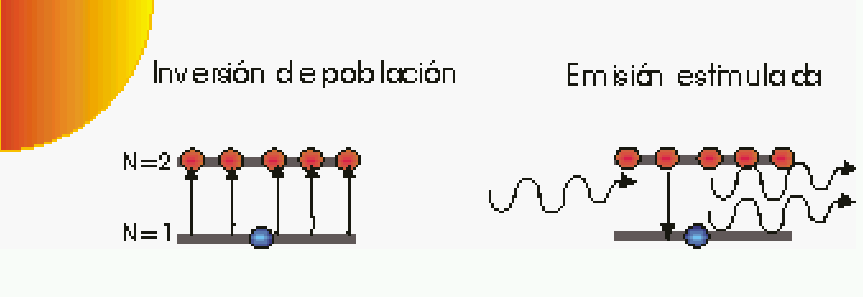
\includegraphics[width=0.7\textwidth,keepaspectratio=true]{./Utils/emision_estimulada.png}
 % emision_estimulada.png: 863x297 pixel, 101dpi, 21.71x7.47 cm, bb=0 0 615 212
 \caption{Inversión de población y emisión estimulada}
 \label{fig:emision_estimulada}
\end{figure}

En la Figura \ref{fig:emision_estimulada} se muestra el proceso de inversi\'on de la poblaci\'on y emisi\'on estimulada. La inversi\'on de la poblaci\'on consiste en excitar los \'atomos de forma que haya m\'as en el nivel de energ\'ia alto que en el bajo, y despu\'es se hace incidir un fot\'on, lo que provoca la emisi\'on de dos fotones con la misma longitud de onda.

\end{itemize}

\subsection{Funcionamiento del m\'aser}

En la Figura \ref{fig:funcionamiento_maser} se describe el funcionamiento del m\'aser. En la imagen las mol\'eculas excitadas, es decir, en un nivel alto de energ\'ia, se representan con c\'irculos rojos, y los peque\~nos c\'irculos azules representan mol\'eculas en un nivel bajo de energ\'ia.

En las im\'agenes A y B vemos c\'omo un grupo de mol\'eculas es excitado por radiaci\'on o choques, de forma que pasan a un nivel alto de energ\'ia. En C un fot\'on incide por la izquierda a estas mol\'eculas. En D, el fot\'on estimula la emisi\'on de la primera mol\'ecula, que libera la energ\'ia retenida en el paso A. Como resultado se obtienen dos fotones de longitud de onda l (en fase) y una mol\'ecula en un nivel bajo de energ\'ia. Estos dos fotones liberados estimulan la emisi\'on de las dos mol\'eculas siguientes (E), en un proceso que contin\'ua en forma de reacci\'on en cadena, doblando el n\'umero de fotones muy r\'apidamente (F).

\begin{figure}[htb!!]
 \centering
 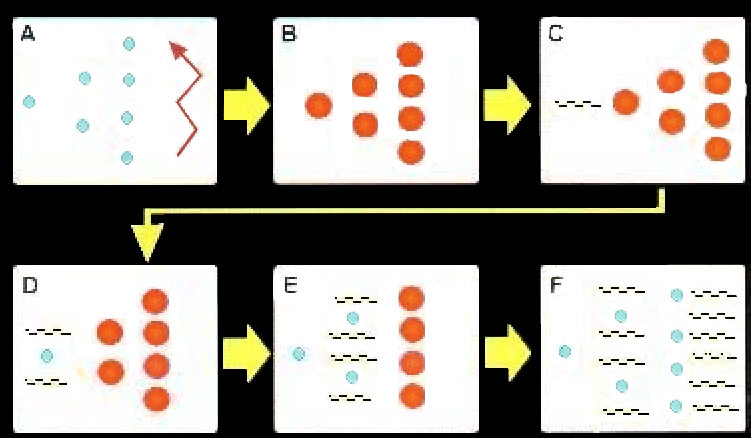
\includegraphics[width=0.9\textwidth]{./Utils/maser_funcionamiento2.png}
 % emision_estimulada.png: 863x297 pixel, 101dpi, 21.71x7.47 cm, bb=0 0 615 212
 \caption{Inversión de población y emisión estimulada}
 \label{fig:funcionamiento_maser}
\end{figure}

Como se ha indicado anteriormente, para que un material produzca emisi\'on m\'aser debe romperse su equilibrio natural. Inyectando energ\'ia en el material se puede conseguir una inversi\'on de la poblaci\'on entre dos niveles, es decir, que haya m\'as \'atomos o mel\'eculas en el nivel de energ\'ia superior. Mientras dura esta inversi\'on, se hace pasar radiaci\'on con la longitud de onda que corresponda a la diferencia de energ\'ia entre dos niveles, y de este modo se estimula una ca\'ida s\'ubita de las part\'iculas del nivel superior al inferior, produciendo un potente fogonazo de microondas. De esta forma se consigue un haz de radiaci\'on intenso, estrecho y monocrom\'atico (es decir, con una \'unica longitud de onda). 

Adem\'as de los m\'aseres artificiales (creados por el hombre), tambi\'en se producen m\'aseres de forma natural en el universo. Son los m\'aseres astron\'omicos, en los que una estrella act\'ua como fuente de energ\'ia, consiguiendo la inversi\'on de la poblaci\'on en un grupo de mol\'eculas. Estos grupos de mol\'eculas son habitualmente nubes moleculares en las que se est\'an formando estrellas o envolturas estelares. Este fen\'omeno nos permite detectar estrellas que de otro modo ser\'ian indetectables porque su emisi\'on espont\'anea es demasiado d\'ebil.

%\newpage
%\input{OtrasTecno.tex}
\newpage
\section{Tipos de M\'aser}
\label{tipos}

Existen tres tipos principales de m\'aser: los de rayo at\'omico, los de gas y los de estado s\'olido. En esta secci\'on hablaremos brevemente de cada uno de estos tres tipos, aunque sin entrar en detalles sobre su funcionamiento a nivel at\'omico.

\subsection{M\'aser de rayo at\'omico}

Los principales m\'aseres de rayo at\'omico son los de hidr\'ogeno y los de amon\'iaco.

\subsubsection{M\'aser de amon\'iaco}

El primer m\'aser, construido por Charles H. Townes y su equipo en la Universidad de Columbia en 1953, utilizaba un haz de mol\'eculas de \textbf{amon\'iaco} para producir la amplificaci\'on de microondas a la frecuencia de 24 GigaHerzios. En la Figura \ref{fig:maser_amoniaco} se muestra la estructura de este tipo de m\'aser \cite{AmoniaMaser}.

\begin{figure}[ht!]
 \centering
 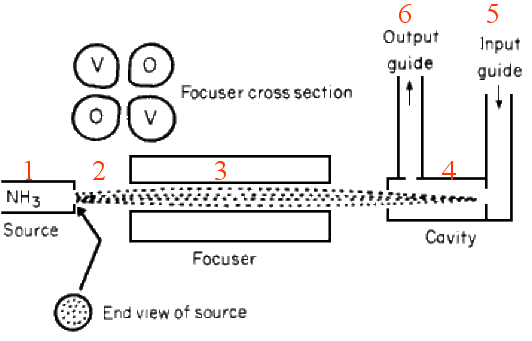
\includegraphics[width=0.6\textwidth]{./Utils/maser_amoniaco.png}
 % maser_hidrogeno.png: 200x375 pixel, 72dpi, 7.06x13.23 cm, bb=0 0 200 375
 \caption{Estructura de un m\'aser de amon\'iaco}
 \label{fig:maser_amoniaco}
\end{figure}

En el m\'aser de amon\'iaco, el gas se calienta primero y las moleculas excitadas se hacen pasar a trav\'es de un campo el\'ectrico no uniforme, de forma que se \textit{recogen} \cite{ElectroAplicado}. Despu\'es las mol\'eculas excitadas pasan a trav\'es de una cavidad, donde ceden su energ\'ia y pasan a su estado de menor energ\'ia. La cesi\'on de energ\'ia se lleva a cabo a trav\'es de una emisi\'on a cierta frecuencia, a la cual la cavidad est\'a sintonizada. Esta frecuencia viene dada por la ley de Planck, y es exactamente 23,87 GHz.



\subsubsection{M\'aser de hidr\'ogeno}
\label{tipo:hidrogeno}

Despu\'es de la creaci\'on del primer m\'aser de amon\'iaco, en 1960 Ramsey y sus colegas de Harvard desarrollaron un máser que funcionaba con hidrógeno y podía utilizarse como un reloj atómico de extremada precisión.

Un m\'aser de hidr\'ogeno, tambi\'en conocido como est\'andar de frecuencia de hidr\'ogeno, es un tipo de m\'aser espec\'ifico que aprovecha las propiedades intr\'insecas del hidr\'ogeno para proporcionar una referencia en frecuencia de precisi\'on. La frecuencia de oscilaci\'on del \'atomo de hidr\'ogeno (su frecuencia de resonancia) es de 1420 MHz.

\begin{figure}[ht!]
 \centering
 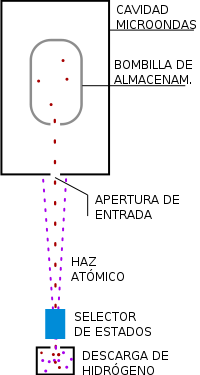
\includegraphics[width=0.33\textwidth]{./Utils/maser_hidrogeno.png}
 % maser_hidrogeno.png: 200x375 pixel, 72dpi, 7.06x13.23 cm, bb=0 0 200 375
 \caption{Estructura de un maser de hidrógeno}
 \label{fig:maser_hidrogeno}
\end{figure}

Los m\'aseres de hidr\'ogeno son dispositivos muy complejos y muy caros. De hecho, es el más costoso de los estándares en frecuencia, y los pocos que existen están en laboratorios internacionales de calibración.

Existen dos tipos de m\'aseres de hidr\'ogeno: activos y pasivos. El m\'aser activo oscila espont\'aneamente y un oscilador de cuarzo se engancha en fase a esta frecuencia de oscilaci\'on. El m\'aser pasivo opera enganchando en frecuencia un oscilador de cuarzo. 



En los dos tipos de m\'aser un peque\~no bote de almacenamiento de hidr\'ogeno molecular (pares de \'atomos de hidr\'ogeno unidos) suelta una cantidad controlada de gas en una cavidad de descarga (ver Figura \ref{fig:maser_hidrogeno}). En esta cavidad las mol\'eculas se separan en \'atomos de hidr\'ogeno individuales mediante un arco. Este hidr\'ogeno at\'omico atraviesa un selector de estado magn\'etico, donde se selecciona el estado deseado antes de hacerlos pasar a la \textit{bombilla} de almacenamiento. Esta bombilla suele tener 20 cm de alto y 10 cm de di\'ametro, y suele estar hecha de cuarzo y revestida de tefl\'on por dentro. Este revestimiento ralentiza la recombinaci\'on de los \'atomos de hidr\'ogeno en mol\'eculas de hidr\'ogeno. 

La bombilla de almacenamiento est\'a situada dentro de una cavidad microondas, que est\'a sintonizada a la frecuencia de resonancia de los \'atomos, 1420 MHz.

Como se ha mencionado antes, en el m\'aser activo la cavidad oscila por s\'i misma. Esto requiere una mayor densidad de \'atomos de hidr\'ogeno y un factor de calidad mayor para la cavidad. El m\'aser activo es m\'as complejo y m\'as caro, pero tiene una mejor estabilidad en frecuencia a largo plazo.

En el m\'aser pasivo, la cavidad se alimenta con una frecuencia externa de 1420 MHz. Esto permite usar una densidad de \'atomos de hidr\'ogeno menor y tambi\'en un menor factor de calidad en la cavidad, lo que reduce el coste.

Ambos tipos de m\'aser poseen mejor estabilidad a corto plazo que los osciladores de cesio. Sin embargo, ya que el comportamiento de un m\'aser de hidr\'ogeno depende de numerosos factores ambientales, posee una incertidumbre en frecuencia mayor que la de los osciladores de cesio, por lo que son peores para medir largos espacios de tiempo.

\subsection{M\'aseres de gas}

El \textbf{m\'aser de rubidio} \cite{rubidium} es un ejemplo de m\'aser de gas utilizado de forma habitual. Al igual que el m\'aser de hidr\'ogeno, sirve como reloj at\'omico. El m\'aser de rubidio es menos preciso, pero tambi\'en menos costoso.

La frecuencia de resonancia del rubidio es 6 834 682 614 Hz, es decir, unos 6,834 GHz. 

El primer est\'andar de frecuencia de rubidio surgi\'o como resultado del trabajo de Carpenter y Arditi en 1960. A\~nos m\'as tarde, en 1964, Davidovits construy\'o el primer m\'aser de rubidio operativo.

El m\'aser de rubidio, al igual que el de hidr\'ogeno, puede funcionar en modo activo o pasivo. El modo pasivo es el m\'as \'util, ya que con un tama\~no menor mantiene una estabilidad en frecuencia excelente. Este dispositivo tiene numerosas aplicaciones en el campo de las comunicaciones, en el espacio y en navegaci\'on, y tiene una estructura similar al m\'aser de hidr\'ogeno.

\subsection{M\'aseres de estado s\'olido}

Los m\'aseres de estado s\'olido \cite{historiaFisica} se basan en hacer transmisiones cu\'anticas en \'atomos con tres niveles de energ\'ia en los cuales el nivel intermedio es metaestable.

La exitosa familia de los\textbf{ m\'aseres de rub\'i} fue iniciada por Chihiro Kukuchi y sus colegas en la Universidad de Michigan. Por su baja temperatura de ruido, los m\'aseres de estado s\'olido encontraron un uso temprano en los radiotelescopios y en antenas de microondas.

\subsection{M\'aseres astron\'omicos}

Adem\'as de los m\'aseres creados por el hombre, existen \textbf{m\'aseres naturale}s presentes en el universo. Estos son los m\'aseres astron\'omicos, que se utilizan para aprender m\'as sobre la composici\'on y constituci\'on del universo. 

Para que en el espacio se produzca una emisi\'on m\'aser \cite{maserEspacio} deben darse como m\'inimo dos condiciones: En primer lugar, tiene que haber la suficiente cantidad de gas para que sus mol\'eculas puedan amplificar la radiaci\'on. En segundo lugar, debe existir una importante fuente de energ\'ia que produzca la inversi\'on de poblaci\'on, es decir, que suba a las mol\'eculas a su nivel de alta energ\'ia. Estas condiciones se dan en diferentes ambientes: regiones de formaci\'on estelar, cometas, atm\'osferas planetarias, estrellas en sus \'ultimas fases de vida e incluso cerca de los agujeros negros centrales de algunas galaxias.

El motivo por el que se produce el efecto m\'aser en estas zonas es que el hidr\'ogeno gaseoso, componente fundamental de la materia interestelar, es especialmente densa en estas regiones. Adem\'as de hidr\'ogeno en la materia interestelar hay otras mol\'eculas, y algunas de ellas act\'uan como amplificadores de radiaci\'on y producen la intensa emisi\'on m\'aser. Los máseres más utilizados en Astronomía son los producidos por el radical hidroxilo, el monóxido de silicio, el metanol y el agua.

La Figura \ref{fig:maser_astronomico} muestra la emisi\'on m\'aser de una estrella en formaci\'on \cite{fotoMaser}. Los c\'irculos blancos representan zonas de emisi\'on m\'aser de la mol\'ecula de agua, que trazan un disco de gas en el que podr\'ia estar form\'andose un nuevo sistema planetario. En color se muestra la emisi\'on en radio de un chorro de material expulsado en direcci\'on perpendicular al disco.

\begin{figure}[ht!]
 \centering
 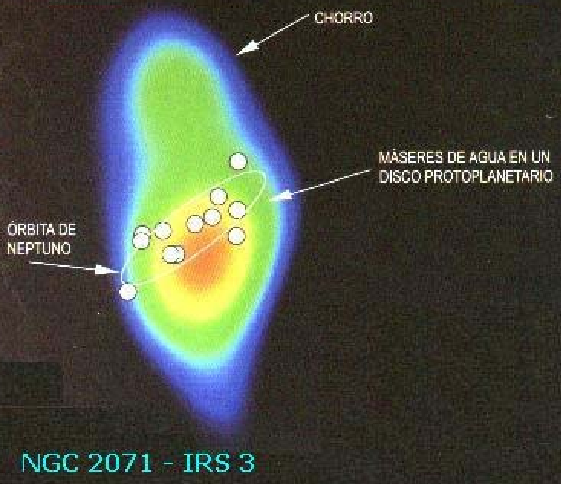
\includegraphics[width=0.6\textwidth]{./Utils/maser_astronomico.png}
 % maser_hidrogeno.png: 200x375 pixel, 72dpi, 7.06x13.23 cm, bb=0 0 200 375
 \caption{Emisi\'on m\'aser de una estrella en formaci\'on}
 \label{fig:maser_astronomico}
\end{figure}

\newpage
\section{Aplicaciones}
\label{aplicaciones}

Los m\'aseres tienen diferentes aplicaciones, principalmente como osciladores (referencias de frecuencia en relojes at\'omicos) y amplificadores de bajo nivel de ruido. En esta secci\'on se describir\'an brevemente estas aplicaciones y otras.

\subsection{Oscilador}

A pesar de la denominaci\'on de amplificadores que tambi\'en se les da, el uso m\'as corriente que se hace de los m\'aseres es como osciladores, sobre todo cuando trabajan a frecuencias elevadas (longitudes de onda submilim\'etricas) para las que, por otra parte, constituyen el \'unico procedimiento pr\'actico de obtener radiaci\'on monocrom\'atica de gran pureza y altas energ\'ias: del orden de GigaVatios (109 GW) en impulsos y de varios centenares de Vatios en onda continua \cite{spiritusTemporis}. 

\subsection{Relojes at\'omicos}
Los m\'asers oscilan a la frecuencia de resonancia del \'atomo o mol\'ecula que los produce con un ancho de banda muy estrecho. Esto hace que sean buenas referencias de frecuencia de alta precici\'on, por lo que sirven, por ejemplo, como relojes at\'omicos. Los m\'aseres de amon\'iaco e hidr\'ogeno se han considerado como patrones de frecuencia y se han utilizado como relojes en experimentos de comprobaci\'on de la relatividad especial.

Un reloj at\'omico es un tipo de reloj que usa una frecuencia de resonancia at\'omica est\'andar como contador. Los primeros relojes at\'omicos eran m\'aseres con cierto equipamiento adicional. Hoy en d\'ia, aunque los m\'aseres se siguen usando en muchos relojes at\'omicos, los est\'andares de frecuencia m\'as avanzados se basan en procesos f\'isicos m\'as avanzados que involucran \'atomos fr\'ios y las fuentes at\'omicas.

El primer reloj at\'omico fue construido en 1949 en la Ofinina Nacional de Normalizaci\'on de los Estados Unidos bas\'andose en las ideas sobre un fen\'omeno extremadamente regular: la resonancia magn\'etica molecular y at\'omica. Sin embargo, la precisi\'on conseguida por el amon\'iaco (mol\'ecula utilizada por este primer prototipo) no era muy superior a los est\'andares de la \'epoca basados en osciladores de cuarzo. En 1955 Louis Essen construy\'o el primer reloj at\'omico realmente preciso en el Reino Unido, bas\'andose en la transici\'on del \'atomo Cesio-133 (que no es un m\'aser). Esto llev\'o a la definici\'on del segundo basada en el tiempo at\'omico. M\'as adelante se crearon m\'aseres de hidr\'ogeno, con una precisi\'on mayor.

La Figura \ref{fig:atomic_clock_gps} muestra un reloj at\'omico hecho a partir de un m\'aser de hidr\'ogeno situado en Canad\'a y perteneciente a la red de posicionamiento global GPS.

\begin{figure}[ht!!]
 \centering
 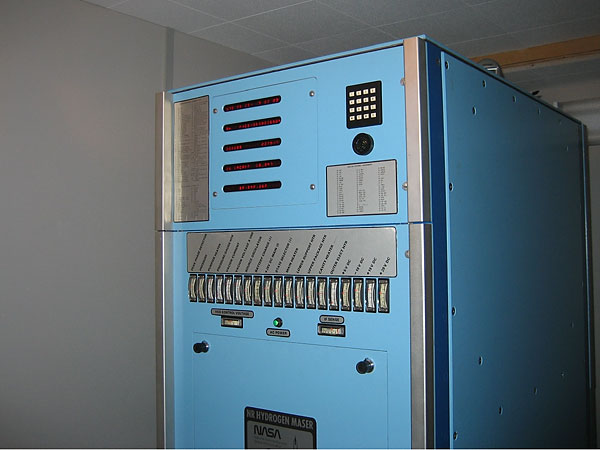
\includegraphics[width=0.5\textwidth]{./Utils/atomic_clock_gps.jpg}
 % atomic_clock_gps.jpg: 600x450 pixel, 100dpi, 15.24x11.43 cm, bb=0 0 432 324
 \caption{Reloj atómico del sistema GPS}
 \label{fig:atomic_clock_gps}
\end{figure}


Dispositivos como los relojes at\'omicos que producen este tipo de mediciones resultan esenciales para la vida moderna. S\'olo gracias a esta exactitud se pueden realizar conexiones v\'ia sat\'elite y funcionan los dispositivos GPS, entre otras cosas. El GPS, de hecho, se basa en dos docenas de satélites, cada uno con cuatro relojes atómicos. Por medio de la triangulación de las señales de tiempo que se emiten desde la órbita, los receptores en el planeta brindan a los usuarios su localización con un alto grado de exactitud.

\subsection{Amplificador de bajo nivel de ruido}

Otra aplicaci\'on de los m\'aseres es la de amplificadores de bajo nivel de ruido, especialmente en radiotelescopios.

Los amplificadores m\'aser tienen un nivel de ruido interno incre\'iblemente bajo, lo que hace que sean extremadamente sensibles. Estas caracter\'isticas hacen que estos dispositivos sean particularmente \'utiles para recepci\'on y detecci\'on de se\~nales muy d\'ebiles en radioastronom\'ia, radiometr\'ia de microondas y aplicaciones similares.

Sin embargo, el uso de amplificadores m\'aser supone un coste elevado, por lo que se utilizan \'unicamente en aquellos casos en que el bajo nivel de ruido requerido justifique el alto coste y la resoluci\'on de los problemas tecnol\'ogicos que surgen, principalmente al tener que utilizar bajas temperaturas. Por ejemplo, se utilizan para detecci\'on de radiaci\'on espacial y comunicaciones con sat\'elites, adem\'as de las aplicaciones mencionadas antes.

La Figura \ref{fig:amplificador_cavidad} muestra un amplificador m\'aser del tipo \textit{cavidad de transmisi\'on}. En amplificadores m\'aser con esta estructura es normal colocar aisladores de ferrita en las gu\'ias de entrada y de salida para proteger al m\'aser de reflexiones que se puedieran producir en la carga. 

\begin{figure}[ht!!]
 \centering
 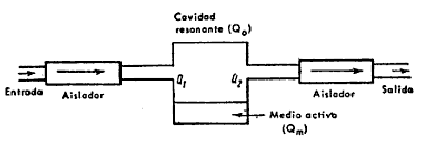
\includegraphics[width=0.7\textwidth]{./Utils/amplificador_transmision.png}
 % atomic_clock_gps.jpg: 600x450 pixel, 100dpi, 15.24x11.43 cm, bb=0 0 432 324
 \caption{Amplificador m\'aser de cavidad de transmisi\'on}
 \label{fig:amplificador_cavidad}
\end{figure}

Como ejemplo de aplicaci\'on pr\'actica, se ha utilizado un amplificador m\'aser en experimentos que detectaban la radiaci\'on c\'osmica generada por el Big Bang que cre\'o el universo.

\subsection{Otras aplicaciones}

Los m\'aseres se utilizan habitualmente como amplificadores, osciladores o relojes at\'omicos. Sin embargo, \'esas no son todas las funciones que pueden cumplir. Por ejemplo, se utilizan en laboratorios para hacer experimentos de mec\'anica cuantica e intentar descubrir nuevas caracter\'isticas de la materia y obtener m\'as informaci\'on sobre los movimientos de los \'atomos. 

Adem\'as, actualmente se est\'an investigando otras posibles aplicaciones de estos dispositivos. El ej\'ercito de los Estados Unidos, por ejemplo, est\'a haciendo pruebas con los m\'aseres como armas disuasorias. Los m\'aseres emiten frecuencias de microondas y, si se apunta con ellos a personas, producen un calentamiento en el agua de la piel. Aunque en principio esto no es peligroso si no se radia durante mucho tiempo a la misma zona, produce una sensaci\'on inc\'omoda en los afectados.

\newpage
\section{Ejemplo de aplicaci\'on pr\'actica}
En esta secci\'on se describir\'a una aplicaci\'on pr\'actica del dispositivo m\'aser: el m\'aser MHM 2010 \cite{MHM2010}, que es un reloj at\'omico de hidr\'ogeno.

\subsection{Caracter\'isticas}
El MHM 2010 es el único maser activo de hidrógeno disponible en el mercado con cavidad independiente. Esto le permite mantener una estabilidad buena durante un largo periodo de tiempo, atributo que únicamente se atribuía a los maseres de cesio.


\begin{figure}[htb!!]
 \centering
 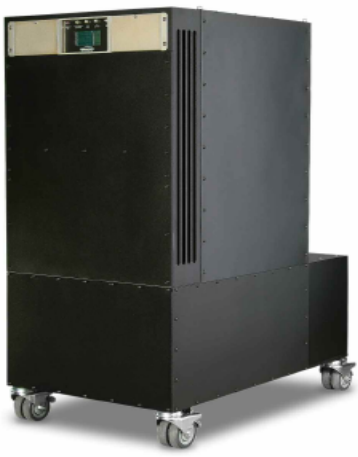
\includegraphics[width=0.3\textwidth]{./Utils/maser_MHM.png}
 % varianzaAllen.png: 607x475 pixel, 101dpi, 15.27x11.95 cm, bb=0 0 433 339
 \label{fig:imagen_maser}
 \caption{M\'aser MHM 2010}
\end{figure}

Este m\'aser puede emitir a tres frecuencias diferentes, teniendo las tres la misma amplitud. En la Tabla \ref{table:amplitud} se muestran las medidas de amplitud tomadas a diferentes frecuencias para una carga de 50 \ohm.

\begin{table}[htb]
\begin{center}
\begin{tabular}[t]{|l|l|}
\hline \hline
\rowcolor[RGB]{244, 184, 184} \textbf{Frecuencia (MHz)} & \textbf{Amplitud (dBm)}\\
\hline \hline
5 & 13\\
\hline
10 & 13\\
\hline
100 & 13\\
\hline\hline
\end{tabular}
\end{center}
\caption{Amplitud del m\'aser a diferentes frecuencias}
\label{table:amplitud}
\end{table}

A medida que aumentamos la frecuencia el ruido de fase va disminuyendo, tal como se muestra en la Tabla \ref{table:ruido_fase}

\begin{table}[htb]
\begin{center}
\begin{tabular}[t]{|l|l|l|}
\hline \hline
\rowcolor[RGB]{244, 184, 184} \textbf{Frecuencia} & \textbf{M\'aser a 5 MHz} & \textbf{M\'aser a 10 MHz}\\
\hline \hline
1 Hz & $\leq$ -112 dBc & $\leq$ -106 dBc\\
\hline
10 Hz & $\leq$ -130 dBc & $\leq$ -124 dBc\\
\hline 
100 Hz& $\leq$ -148 dBc & $\leq$ -142 dBc\\
\hline 
1 KHz& $\leq$ -155 dBc & $\leq$ -149 dBc\\
\hline 
10 KHz& $\leq$ -155 dBc & $\leq$ -149 dBc\\
\hline
100 KHz& $\leq$ -155 dBc & $\leq$ -149 dBc\\
\hline\hline
\end{tabular} 
\end{center}
\caption{Ruido de fase del m\'aser en funci\'on de la frecuencia}
\label{table:ruido_fase}
\end{table}


Como se ha dicho al principio de este punto, este m\'aser presenta una buena estabilidad, incluso tras haber transcurrido un largo tiempo. En la Figura \ref{fig:varianza_allan} se muestra la caracter\'istica de este oscilador (su varianza de Allan\footnote{Para caracterizar la estabilidad en frecuencia de los osciladores se utiliza la varianza de Allan, porque no presenta ambigüedades ni inconsistencias en su caracterizaci\'on. }), mostrando el tiempo en el eje \textit{x} y la desviaci\'on producida en el eje \textit{y}.

\begin{figure}
 \centering
 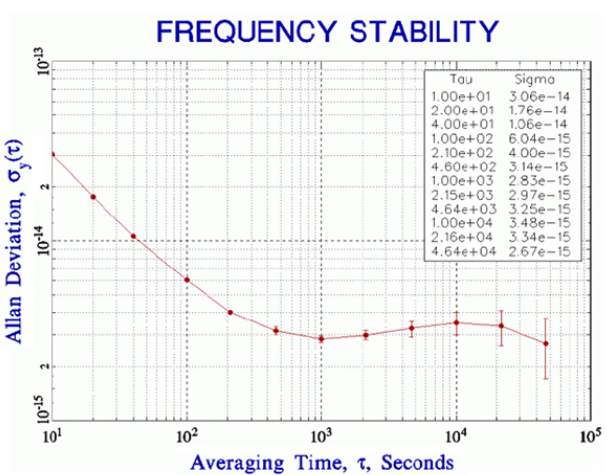
\includegraphics[width=0.8\textwidth]{./Utils/varianzaAllen.png}
 % varianzaAllen.png: 607x475 pixel, 101dpi, 15.27x11.95 cm, bb=0 0 433 339
 \caption{Estabilidad en frecuencia del oscilador}
 \label{fig:varianza_allan}
\end{figure}

Este m\'aser funciona con un voltaje comprendido entre 85 y 264 VAC, de 47 a 63 Hz de frecuencia. Si trabaja con continua requiere de 22 a 28 voltios con una intensidad típica de 3.1 amperios. En este caso tiene un tiempo de trabajo de 8 horas.

\subsection{Funcionamiento}

A continuaci\'on se explica el funcionamiento de este m\'aser de hidr\'ogeno a partir de su diagrama de bloques (ver Figura  \ref{fig:maser_desglosado}). Para simplificar el diagrama se han destacado \'unicamente las partes propias del m\'aser, dejando de lado las de control. 

\begin{figure}[hb!!!]
 \centering
 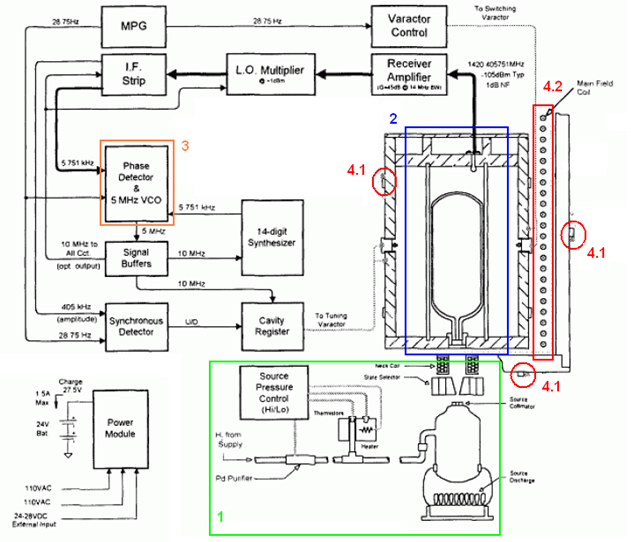
\includegraphics[width=\textwidth]{./Utils/maser_desglosado.png}
 % varianzaAllen.png: 607x475 pixel, 101dpi, 15.27x11.95 cm, bb=0 0 433 339
 \caption{Esquema del funcionamiento del maser}
 \label{fig:maser_desglosado}
\end{figure}

1. Fuente de hidrógeno y puertas magnéticas que permiten el paso de ciertas moléculas.

2. Cavidad de resonancia.

3. PLL y VCO para generar la señal de salida.

4. Control de temperatura. Para ello se realiza mediante termistores (4.1), que son resistencias cuyo valor varía con la temperatura, y un escudo térmico (4.2).


Para explicar mejor su funcionamiento se prestará mayor atención a la Figura \ref{fig:esquema_maser}, ya que visualiza esquemáticamente las partes involucradas.

\begin{figure}[hb!!]
 \centering
 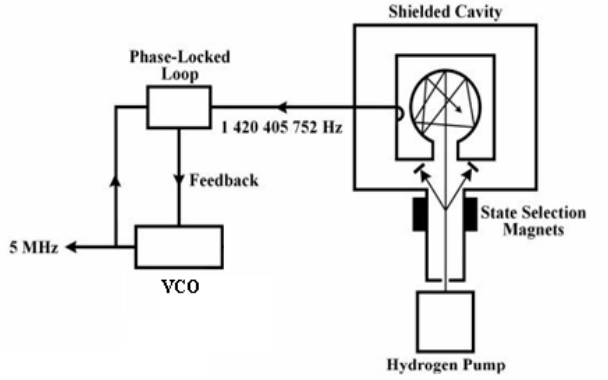
\includegraphics[width=0.7\textwidth]{./Utils/maser_esquema.png}
 % varianzaAllen.png: 607x475 pixel, 101dpi, 15.27x11.95 cm, bb=0 0 433 339
 \caption{Esquema del m\'aser}
 \label{fig:esquema_maser}
\end{figure}

Como se ha explicado en el punto \ref{tipo:hidrogeno}. \nameref{tipo:hidrogeno}, los m\'asers de hidrogeno funcionan a la frecuencia de resonancia del átomo de hidrógeno, que es 1420 MHz. 

Un máser de hidrógeno funciona mediante el envío de gas de hidrógeno a través de una puerta magnética que sólo permite que los átomos con cierta energía pasen a través. 

Los átomos que atraviesan la puerta entran en una bombilla de almacenamiento rodeada por una cavidad resonante. Una vez dentro de la bombilla, cuando alcanzan un estado energético menor, liberan fotones a frecuencias de microondas. Estos fotones estimulan otros átomos a abandonar su nivel de energía, y ellos a su vez liberan más fotones. De esta manera, un campo de microondas autosostenible se acumula en la bombilla. La cavidad resonante que rodea la bombilla ayuda a redirigir a los fotones de nuevo al sistema para mantener la oscilación. El resultado es una señal de microondas de la frecuencia de resonancia del átomo de hidrógeno y que continuamente se emiten en función del tiempo que lleve la entrada de nuevos átomos al sistema.

Una vez generada la señal de microondas a 1420 MHz se introduce en un oscilador basado en un PLL (sistema enganchado en fase). El m\'aser dispone de un VCO que oscila a una frecuencia determinada (frecuencia de oscilación libre), que se compara con la que se ha generado en la cavidad de resonancia. Al realizar dicha comparación se generan productos de las frecuencias, que se har\'an pasar por un filtro para delimitar la frecuencia deseada.

La frecuencia de salida puede ser modificada variando la tensión de entrada del VCO, ya que al variar su tensión se var\'ia la frecuencia a la que oscila.

\newpage
%\input{Curiosidades.tex}
%\newpage
\section{Conclusiones}
\label{conclusiones}

Un m\'aser es un \textbf{dispositivo que produce ondas electromagn\'eticas coherentes} mediante la amplificaci\'on por la emisi\'on estimulada de radiaci\'on. El t\'ermino se defini\'o como acr\'onimo de \textit{Microwave Amplification by Stimulated Emission of Radiation}, aunque es aplicable a un mayor rango de frecuencias, no s\'olo a las ondas de microondas.

El funcionamiento de los m\'aseres se basa en el fen\'omeno de la \textbf{emisi\'on estimulada de radiaci\'on}. En primer lugar se produce una inversi\'on de poblaci\'on de los \'atomos o mol\'eculas, es decir, se les excita para llevarlos a su nivel de energ\'ia superior. Despu\'es se hace incidir un fot\'on de una longitud de onda determinada, lo que produce que la mol\'ecula afectada baje a su nivel inicial de energ\'ia emitiendo dos fotones de la misma longitud de onda. Este fen\'omeno produce una reacci\'on en cadena que hace que se liberen r\'apidamente muchos fotones coherentes y con la misma longitud de onda.

Los m\'aseres producen \textbf{radiaci\'on coherente monocrom\'atica}, es decir, con una frecuencia muy estrecha, por lo que son adecuados como osciladores y como relojes at\'omicos. De hecho, algunos tipos de m\'aseres se usan como est\'andares temporales (como el m\'aser de hidr\'ogeno). Debido a su bajo nivel de ruido, los m\'aseres tambi\'en se utilizan como amplificadores en ciertos sistemas con requerimientos muy especiales, como en radiotelescopios.

Adem\'as de los m\'aseres creados por el hombre, ya exist\'ian en la naturaleza algunos naturales: son los \textbf{m\'aseres astron\'omicos}, que se producen en el espacio, especialmente en zonas donde se est\'an formando estrellas, y que permiten a los cient\'ificos obtener informaci\'on sobre el universo en que vivimos.

 
% CONFIG: Estilo de la bibliograf�a
\pretolerance=10 %Para evitar que se corten las palabras
\tolerance=10  %Para evitar que se corten las palabras
\cleardoublepage                                  % empezar en p�gina a la derecha
\addcontentsline{toc}{section}{REFERENCIAS} % as� aparecer� en el ToC principal como "Bibliograf�a"
\bibliographystyle{unsrt}                          % el estilo de bibliograf�a. unsrt: números en orden, plain: números, alpha para nombre del autor y año

% CONTENIDO: Bibliografia. Introduce una lista de ficheros .bib que quieras usar, como se expone.
\newpage
\bibliography{file-bibliography}

\newpage
\thispagestyle{empty}
\begin{textblock*}{200mm}(10mm,25mm)
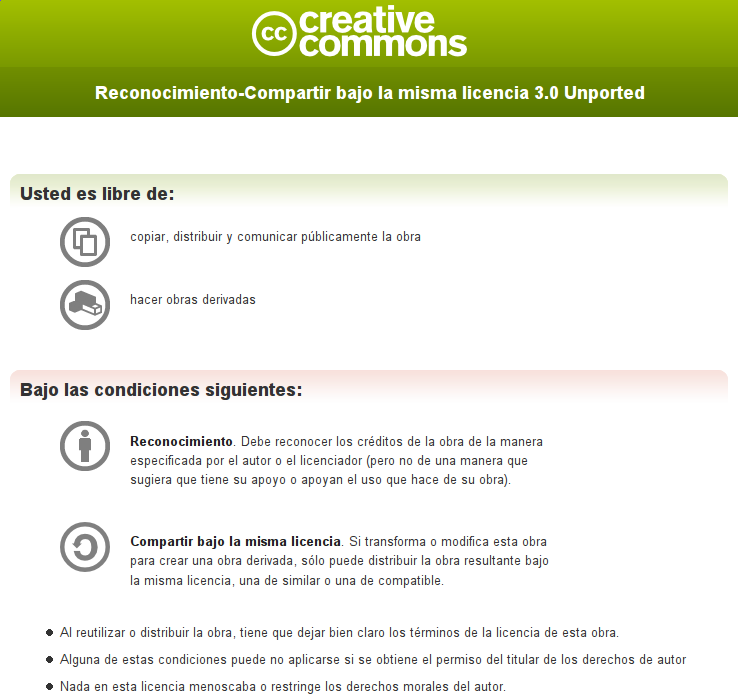
\includegraphics[height=170mm]{Utils/licencia-by-sa.png}
\end{textblock*}
 

\end{document}
